\section{Язык Дика и двунаправленные графы}\label{section:bidirected}

В данной главе будет рассмотрена модификация алгоритма~\ref{algo:PI}, основанная на ослаблении условия на граф, а именно, на ``предположении'', что он является неориентированным. Также будет доказана корректность данной модификации для двунаправленных графов и языка Дика, а также для неориентированных графов и некоторых видов грамматик.

Для неориентированных графов отношение достижимости равно отношению ``принадлежать одной компоненте связности''. Поддерживать добавление рёбер и проверку связности в неориентированном графе можно с помощью структуры данных Система Непересекающихся Множеств. 

% Система Непересекающихся Множеств (СНМ)
\begin{definition}\label{def:DSU}
  \textit{Система Непересекающихся Множеств (или СНМ)}\footnote{Disjoint-set/union–find data data structure}~\cite{Galler1964}~--- структура данных для работы с непересекающимися множествами. Её интерфейс включает следующие операции:
  \vspace{-\topsep}
  \begin{itemize}
    \setlength\itemsep{-0.1em}
    \item \textit{MakeSet}$(x)$~--- создаёт новое множество, состоящее из одного элемента $x$.
    \item \textit{Find}$(x)$~--- возвращает элемент-представитель множества, содержащего $x$.\\ Для всех элементов одного множества элемент-представитель одинаков.
    \item \textit{Union}$(x, y)$~--- объединяет множества, содержащие элементы $x$ и $y$.
  \end{itemize}
\end{definition}

\subsection{Алгоритм, основанный на неориентированном транзитивном замыкании}

В листинге~\ref{algo:NP} приведён псевдокод алгоритма.

\begin{algorithm}[h]
  \floatname{algorithm}{Listing}
  \begin{algorithmic}[1]
  \caption{Алгоритм достижимости для РКА, основанный на неориентированном ИТЗ}
  \label{algo:NP}
  \Function{UndirectedRSMReachability}{$\cool{R}$}
      \State{$A \gets$ Empty adjacency matrix}
      \State{$Q \gets$ Empty Queue}
      \State{$D \gets$ DSU($|\bigcup\limits_{i=1}^k Q_i|$)}
      \For{$i \in 1..k$}
          \For{$u \xrightarrow{c} v \in \delta_i$}
              \State{$Q.Push(\q{u, v, i})$}
          \EndFor
      \EndFor
      \While{$Q$ is not Empty}
          \State{$\q{u, v, i} \gets Q.Pop()$}
          \If{$u \in En_i \wedge v \in En_i$}
              \Comment{Нашли новый путь}
              \State{$A \gets A \cup getEdges(i, u, v)$}
              \State{$Q.PushAll(getEdges(i, u, v))$}
              \State{$D.Union(u, v)$}
              \Comment{Добавляем новые рёбра}
          \EndIf
      \EndWhile
  \State \Return $A$
  \EndFunction
  \end{algorithmic}
\end{algorithm}

Для реализации используются две вспомогательные структуры данных: очередь $Q$, хранящая рёбра, которые были добавлены в граф, но ещё не обработаны (как и в оригинальном алгоритме), и СНМ $D$, поддерживающая компоненты связности и поиск новых путей $\langle$стартовое состояние$\to$конечное состояние$\rangle$. 

Опишем подробно структуру используемой СНМ (в листинге~\ref{algo:DSU} приведён псевдокод).

\algblockdefx[Structure]{Structure}{EndStructure}
[1]{{\bf Structure} #1}
{}

\begin{algorithm}[h]
  \floatname{algorithm}{Listing}
  \begin{algorithmic}[1]
  \caption{Система Непересекающихся Множеств}
  \label{algo:DSU}
  \Structure{DisjointSets}
      \Function{DisjointSets}{$V$}
          \For{$v \in V$}
              \State{$P[v] \gets v$}
              \Comment{Предкок}
              \State{$R[v] \gets 0$}
              \Comment{Ранг}
          \EndFor
          \For{$v \in En(V)$}
              \State{$En[v] \gets \{v \}$}
              \Comment{Список стартовых вершин поддерева}
          \EndFor
          \For{$v \in Ex(V)$}
              \State{$Ex[v] \gets \{v \}$}
              \Comment{Список конечных вершин поддерева}
          \EndFor
      \EndFunction
      \Function{Find}{$v$}
          \If{$P[v] = v$}
              \Return $v$
          \EndIf
          \Return $P[v] = Find(P[v])$
          \Comment{Эвристика сжатие путей}
      \EndFunction
      \Function{Union}{$u, v$}
          \State{$u \gets Find(u)$}
          \State{$v \gets Find(v)$}
          \If{$u = v$}
              \Return
          \EndIf
          \If{$R[u] > R[v]$}
              \State{$Swap(u, v)$}
              \Comment{Ранговая эвристика}
          \EndIf
          \State{$Q.PushAll(\{ \q{en_u, ex_v}~|~en_u \in En[u], ex_v \in Ex[v] \})$}
          \State{$Q.PushAll(\{ \q{en_v, ex_u}~|~en_v \in En[v], ex_u \in Ex[u] \})$}
          \Comment{Добавление новых рёбер}
          \State{$En[v] \gets En[v] \cup En[u]$}
          \State{$Ex[v] \gets Ex[v] \cup Ex[u]$}
          \State{$R[v] \gets \max(R[v], R[u]+1)$}
          \State{$P[u] = v$}
          \Comment{Объединение компонент}
      \EndFunction
  \EndStructure
  \end{algorithmic}
\end{algorithm}

За основу взята стандартная реализация \cite{Hopcroft1973} на подвешенных деревьях, использующая обе эвристики: сжатие путей и ранговую. 

Дополнительно в корнях хранятся списки всех начальных и конечных состояний компоненты. При добавлении ребра в операции \textit{Union} перебираются все пары начальная/конечная вершина из двух компонент и соответствующие им рёбра добавляются в рабочую очередь $Q$. 

% \TODO: (подумоть) можно ли добавлять сразу много рёбер и сжимать их дфсом (как Борувка)?

\subsection*{Время работы}

\begin{theorem}
  На РКА из $|V|$ состояний и $|E^{*}|$ рёбрах в транзитивном замыкании, алгоритм~\ref{algo:NP} отработает за время $\O(|V| + |E^{*}| \alpha(|V|))$
\end{theorem}

\begin{proof}
  Как и в алгоритме~\ref{algo:PI} проход по внешнему циклу и добавление новых рекурсивных рёбер отработает за $\O(|E^{*}|)$, так как каждое ребро транзитивного замыкания рассмотрится не более одного раза.

  Осталось оценить время работы $|E^{*}|$ вызовов функции \textit{Union}. Каждый из них совершает 2 вызова функции \textit{Find}, каждый из которых отработает за амортизированное $\O(\alpha(|V|))$. Также, если вершины находились в разных компонентах, происходит перебор всех пар начальное-конечное состояние. Однако, этот перебор суммарно переберёт каждое ребро транзитивного замыкания не более одного раза, так что суммарно отработает за $\O(|E^{*}|)$.

  Итого, время работы алгоритма составляет $\O(|V| + |E^{*}| \alpha(|V|))$ ($\O(|V|)$ берётся из создания СНМ на $|V|$ множеств). 
\end{proof}

\begin{note}
  Алгоритм~\ref{algo:NP} очевидно работает корректно на РКА, все рёбра которого неориентированы. Вспомним, что для решения задачи CFPQ алгоритм достижимости запускается на прямом произведении входного графа и РКА входной грамматики. Так что, чтобы произведение было неориентированным, необходима неориентированность и входного графа и РКА входной грамматики. 

  И если неориентированные графы являются довольно естественными объектами, то неориентированные РКА задают очень специфичные языки (про языки, задаваемые неориентированными НКА можно почитать в~\cite{Kutrib18}). 

  Так что в следующем разделе будет показана корректность алгоритма~\ref{algo:NP} для более реалистичного частного случая.
\end{note}

\subsection{Корректность для двунаправленных графов и языка Дика}

\begin{theorem}\label{th:bidir_corr}
  Алгоритм~\ref{algo:NP} работает корректно на двунаправленных графах и языке Дика.
\end{theorem}

Для доказательства потребуется следующее вспомогательное утверждение:

\begin{lemma}\label{lemma:bidir_equiv}
  Для вершин двунаправленных графов отношении Диковой достижимости является отношением эквивалентности.
\end{lemma}
\begin{proof}

  Действительно, если инвертировать (заменить все $(_i$ на $)_i$ и наоборот) и развернуть правильную скобочную последовательность, то получится так же правильная скобочная последовательность.\\
  Пример: ПСП: `\texttt{([]())}' $\to$ развёрнутая: `\texttt{))(][(}' $\to$ инвертированная: `\texttt{(()[])}'.

\end{proof}

\begin{adjustbox}{valign=T,raise=\strutheight,minipage={\linewidth}}
  \begin{wrapfigure}{r}{0.47\linewidth}
    \begin{tikzpicture}[shorten >=1pt,auto]
       \node[state, initial]   (q_1)                      {$1$};
       \node[state]            (q_2)  [above right=of q_1] {$2$};
       \node[state, accepting] (q_3)  [right=of q_2]       {$3$};
       \node[state]            (q_4)  [right=of q_1]       {$4$};
       \node[state]            (q_5)  [right=of q_4]       {$5$};
       \node[state, accepting] (q_6)  [right=of q_5]       {$6$};
       \node[state]            (q_7)  [below right=of q_1] {$7$};
       \node[state]            (q_8)  [right=of q_7]       {$8$};
       \node[state, accepting] (q_9)  [right=of q_8]       {$9$};
       \node[state, accepting] (q_10) [below=of q_8]       {$10$};
        \path[->]
        (q_1) edge[above, thick] node {$S$} (q_2)
        (q_2) edge[above, thick] node {$S$} (q_3)
        (q_1) edge[above, thick] node {$(_1$} (q_4)
        (q_4) edge[above, thick] node {$S$} (q_5)
        (q_5) edge[above, thick] node {$)_1$} (q_6)
        (q_1) edge[below, thick] node {$(_2$} (q_7)
        (q_7) edge[above, thick] node {$S$} (q_8)
        (q_8) edge[above, thick] node {$)_2$} (q_9)
        (q_1) edge[bend right, below, thick] node {$\eps$} (q_10);
    \end{tikzpicture}
    \caption{РКА для языка Дика $\cool{D}_2$.\\ Состоит из одной компоненты $S$.}
    \label{img:dyck_rsm}
  \end{wrapfigure}

  \strut{}

  \begin{note}
    В доказательстве для простоты будет рассматриваться язык Дика $\cool{D}_2$ (на двух типах скобок). Все рассуждения обобщаются на случай $k$ типов скобок.
  \end{note}

  \begin{note}    
    Для данного алгоритма будем использовать не совсем стандартный РКА для языка Дика (изображён на рис.~\ref{img:dyck_rsm}). Нестандартность заключается в том, что он содержит несколько (а именно, $k + 2$) терминальных состояний, тогда как обычно они объединены в одну вершину.
  \end{note}

\end{adjustbox}

\begin{proof}{Теоремы~\ref{th:bidir_corr}}

  Достаточно доказать, что для любой пары состояний $e \in En_i, ex \in Ex_i$ существование неориентированного пути эквивалентно существованию ориентированного.

  $\Leftarrow$ (ориентированный $\SO$ неориентированный)

  Очевидно, если есть ориентированный путь $en \path ex$, то если убрать ориентацию этот путь всё ещё останется корректным.

  $\Rightarrow$ (неориентированный $\SO$ ориентированный)

  Для начала заметим, что компонента нашего РКА (произведения РКА языка Дика и входного графа) образует слоистую структуру: на $i$-ом слое~--- состояния $\q{q_i, u}$, где $q_i$~--- $i$-ое состояние РКА языка Дика. Т.к. РКА Дика топологически отсортирован, все рёбра ведут из слоя с меньшим номером в слой с большим.

  Назовём неориентированный путь \textit{простым}, если он проходит по каждому слою не боле одного раза.

  Пусть есть неориентированный путь $p \colon en \path ex$. Покажем, что тогда существует \textit{простой} путь $p' \colon en \path ex$. Заметим, что так как рёбра идут только из слоя с меньшим номером в слой с большим, то простой путь из первого слоя в последний на самом деле направлен согласно исходной ориентации рёбер. Т.е. такой простой путь и будет искомым.

  Доказывать это утверждение (про наличие простого пути $p'$) будем индукцией по длине пути.

  Очевидно, утверждение верно для путей длины 1, 2 и 3~--- все они и так являются простыми.

  Рассмотрим путь $p$ длины $\ge 4$, он уже не будет простым. Найдём первую \textit{точку перегиба} пути~--- вершину, из который путь идёт в состояние на слое с меньшим номером.

  Внимательно посмотрев на РКА языка Дика, можно заметить, что все состояния имеют входящую степень 1 (для этого и нужен был нестандартный вид), так что рёбра, соседствующие в пути $p$ с точкой перегиба имеют одинаковую метку и идут на один и тот же уровень. Обозначим эти рёбра как $\q{q_i, u} \to \q{q_j, v} \to \q{q_i, w}$ ($\q{q_j, v}$~--- точка перегиба).

  Рассмотрим все 3 варианта возможной метки на рёбрах вокруг точки перегиба.

  \begin{itemize}
    \item открывающая скобка $(_k$

      $p \colon (q_1, u) \rightarrow (q_{4/7}, v) \rightarrow (q_1, w) \rightarrow \dots \rightarrow (q_f, z)$.

      Рёбра с меткой $(_k$ соответствуют рёбрам входного графа, а именно рёбрам $u \xrightarrow{(_k)} v$ и $w \xrightarrow{(_k)} v$. Заметим, что тогда, по двунаправленности графа, существует и ребро $v \xrightarrow{)_k} w$, дающее вместе с ребром $u \xrightarrow{(_k)} v $ путь $(_k )_k$ из $u$ в $w$, порождающий $S$-ребро $\q{q_1, u} \to \q{q_2, w}$. Также, по предположению индукции существует простой путь $\q{q_1, w} \to \q{q_f, z}$, а значит есть и $S$-ребро $\q{q_2, w} \to \q{q_3, z}$. Вместе эти два ребра формируют просто путь $\q{q_1, u} \to \q{q_2, w} \to \q{q_3, z}$, что и хотелось.

    \item $S$-метки

      $p \colon (q_1, a) \rightarrow \dots \rightarrow (q_i, u) \rightarrow (q_j, v) \rightarrow (q_i, w) \rightarrow \dots \rightarrow (q_f, z)$.

      По лемме~\ref{lemma:bidir_equiv}, из наличия дикового пути $w \path v$ следует наличие дикового пути $v \path w$. Вместе два диковых пути $u \path v$ и $v \path w$ образуют один путь $u \path w$. 

      Сожмём этот путь в одну вершину $uw$. Получим более короткий путь, для него по предположению индукции существует аналогичный простой путь. Если этот простой путь не проходит через вершину $uw$, то он и является ответом. Иначе. Если вершина $uw$ находится на 2, 4 или 7 слое, то следующее за ней ребро в простом пути имеет метку $S$, а значит, вместе с диковым путём $u \path w$ собирается в один диков путь (по правилу $S \to SS$, как в случае $(_k$). Если же $uw$ находится на 1 слое, то весь путь от неё до $z$~--- один диков путь, который так же складывается с путём $u \path w$.  

    \item закрывающая скобка $)_k$

      $p \colon (q_1, a) \rightarrow \dots \rightarrow (q_i, u) \rightarrow (q_f, v) \rightarrow (q_i, w) \rightarrow \dots \rightarrow (q_f', z)$.

      По предположению индукции, существует простой путь $a \path v$, так что есть $S$-ребро $\q{q_1, a} \to \q{q_2, v}$. Поймём, почему будет и ребро $\q{q_2, v} \to \q{q_3, z}$, которое вместе с предыдущем даёт искомый простой путь.

      По двунаправленности графа, из наличия ребра $w \xrightarrow{)_k} v$ следует наличие ребра $v \xrightarrow{(_k)} w$. Вместе с изначальным $\eps$-ребром $w \xrightarrow{S} w$ и остатком пути $\q{q_i, w} \path \q{q_f', z}$ получаем более короткий путь, для которого, по предположению индукции существует аналогичный простой путь. Он и порождает второе ребро $\q{q_2, w} \to \q{q_3, z}$. 

    \begin{figure}[H]
        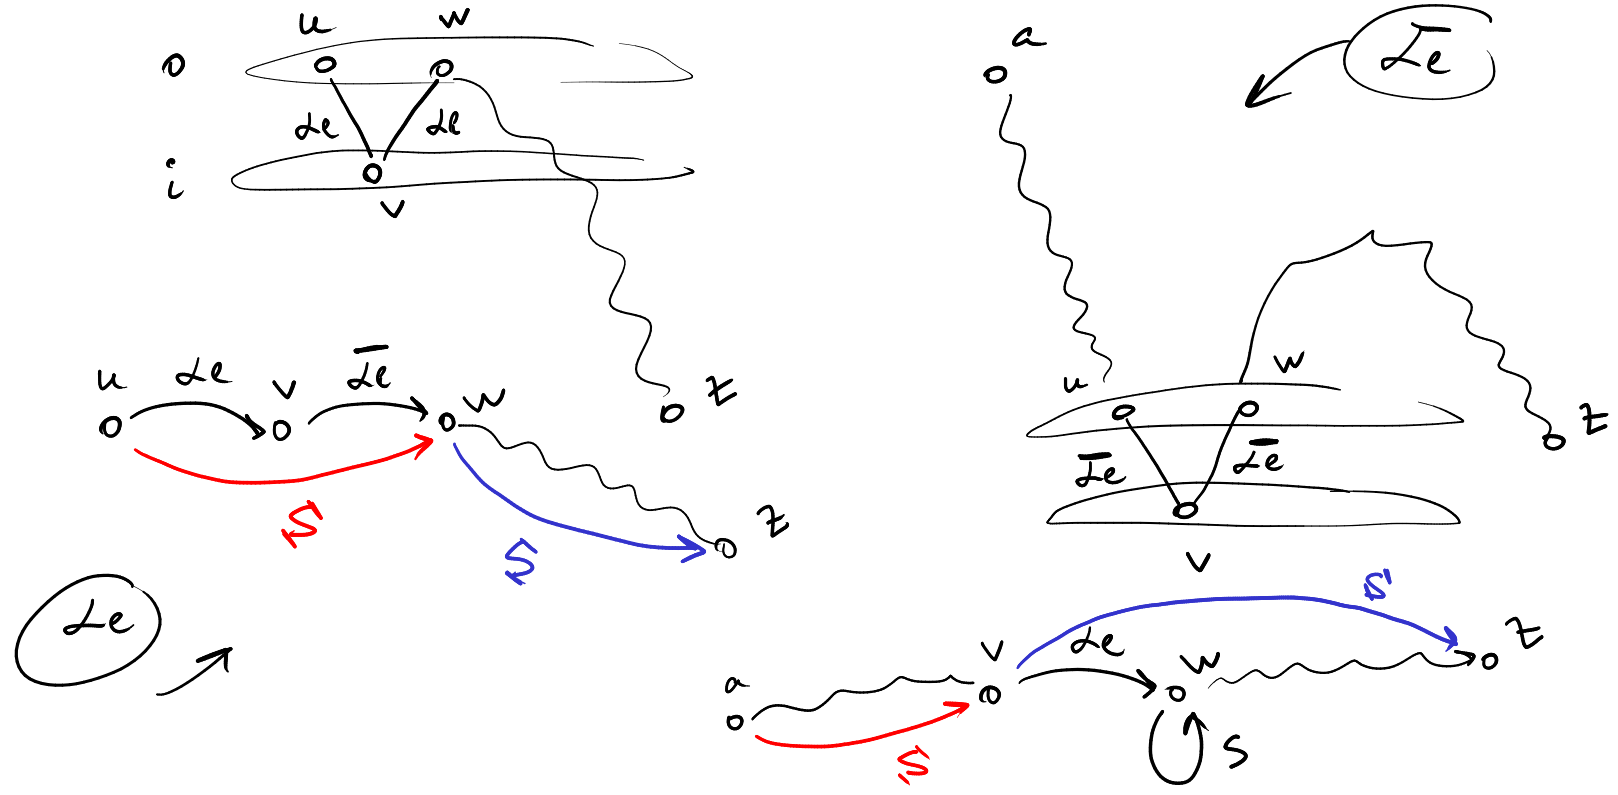
\includegraphics[width=\linewidth]{img/th_proof_img}
    \end{figure}

    \TODO: норм картинка
  \end{itemize}

\end{proof}

\subsection{Выводы и результаты {}по главе}

В этой главе была представлена модификация алгоритма~\ref{algo:PI}, предполагающая неоринтированность данного ей РКА. Алгоритм~\ref{algo:NP} использует структуру данных СНМ~\ref{def:DSU} для поддержания инкрементального транзитивного замыкания неориентированного графа. Также была доказана корректность данного алгоритма для двунаправленных графов и языка Дика.

% 
\includegraphics[width=0.75\linewidth]{img/hole}
